% arara: lualatex: { shell: true }
% arara: biber
% arara: lualatex: { shell: true }
% arara: lualatex: { shell: true, synctex: true }
\RequirePackage{luatex85}
\documentclass[aspectratio=169,hyperref={pdfpagelabels=false,pageanchor=false,bookmarks=false}]{beamer}

% Math support
\usepackage{mathtools,amssymb}

% Beamer theme
\useoutertheme[progressbar=frametitle,numbering=fraction]{metropolis}
\useinnertheme{metropolis}
\usefonttheme{professionalfonts}
\usecolortheme{metropolis}

% Fonts
\usepackage[no-math]{fontspec}
\usepackage{microtype}
\defaultfontfeatures{Ligatures=TeX}
% open source alternative to Gill Sans in UU's official layout
\usepackage[sfdefault]{gillius2}
\newfontfamily\JuliaMono{JuliaMono-Regular.otf}[
Path=../shared/fonts/,
Extension=.ttf
]
\newfontface\JuliaMonoMedium{JuliaMono-Regular}
\setmonofont{JuliaMonoMedium}[Contextuals=Alternate, Scale=MatchLowercase]
\usepackage[OT1,euler-digits]{eulervm}
\setbeamerfont{title}{size=\Large,series=\bfseries}
\setbeamerfont{author}{size=\small}
\setbeamerfont{date}{size=\small}
\setbeamerfont*{subtitle}{size=\large}
\setbeamerfont{frametitle}{size=\large,series=\bfseries}
\setbeamerfont{footnote}{size=\tiny}
\setbeamerfont{page number in head/foot}{size=\tiny}
\setbeamerfont{standout}{size=\Large,series=\bfseries}

% Languages
\usepackage{polyglossia}
\setdefaultlanguage{english}
\usepackage{csquotes}

% Graphics
\usepackage{graphicx}
\usepackage[export]{adjustbox}

% Tables
\usepackage{booktabs}

% Colors
\def\UseCMYK{true}
\ifdefined\UseCMYK
	\definecolor{uured}{cmyk}{0.07,1.00,0.82,0.26}
\else
	\definecolor{uured}{RGB}{166,25,46}
\fi

\ifdefined\UseCMYK
	\definecolor{black}{cmyk}{0.00,0.00,0.00,1.00}
\else
	\definecolor{black}{RGB}{0,0,0}
\fi

\colorlet{uulightgrey}{black!10}
\colorlet{uumidgrey}{black!30}
\colorlet{uudarkgrey}{black!50}

% Pantone 483
\ifdefined\UseCMYK
	\definecolor{mull}{cmyk}{0.21,0.80,0.81,0.69}
\else
	\definecolor{mull}{RGB}{101,48,36}
\fi
\colorlet{mullstark}{mull!30}
\colorlet{mullmellan}{mull!20}
\colorlet{mullsvag}{mull!10}

% Pantone 1675
\ifdefined\UseCMYK
	\definecolor{sand}{cmyk}{0.05,0.83,0.100,0.27}
\else
	\definecolor{sand}{RGB}{169,67,30}
\fi
\colorlet{sandstark}{sand!30}
\colorlet{sandmellan}{sand!20}
\colorlet{sandsvag}{sand!10}


% Pantone 131

\ifdefined\UseCMYK
	\definecolor{blond}{cmyk}{0.02,0.39,1.00,0.10}
\else
	\definecolor{blond}{RGB}{204,138,0}
\fi
\colorlet{blondstark}{blond!30}
\colorlet{blondmellan}{blond!20}
\colorlet{blondsvag}{blond!10}



% Pantone 7546
\ifdefined\UseCMYK
	\definecolor{skugga}{cmyk}{0.73,0.45,0.24,0.66}
\else
	\definecolor{skugga}{RGB}{37,55,70}
\fi
\colorlet{skuggastark}{skugga!30}
\colorlet{skuggamellan}{skugga!20}
\colorlet{skuggasvag}{skugga!10}

% Pantone 534
\ifdefined\UseCMYK
	\definecolor{skymning}{cmyk}{0.95,0.75,0.07,0.44}
\else
	\definecolor{skymning}{RGB}{37,54,93}
\fi
\colorlet{skymningstark}{skymning!30}
\colorlet{skymningmellan}{skymning!20}
\colorlet{skymningsvag}{skymning!10}

% Pantone 645
\ifdefined\UseCMYK
	\definecolor{gryning}{cmyk}{0.56,0.21,0.02,0.08}
\else
	\definecolor{gryning}{RGB}{125,161,196}
\fi
\colorlet{gryningstark}{gryning!30}
\colorlet{gryningmellan}{gryning!20}
\colorlet{gryningsvag}{gryning!10}

% Pantone 7484
\ifdefined\UseCMYK
	\definecolor{gronska}{cmyk}{0.91,0.14,0.78,0.60}
\else
	\definecolor{gronska}{RGB}{0,87,63}
\fi
\colorlet{gronskastark}{gronska!30}
\colorlet{gronskamellan}{gronska!20}
\colorlet{gronskasvag}{gronska!10}

% Pantone 7494
\ifdefined\UseCMYK
	\definecolor{skir}{cmyk}{0.35,0.05,0.42,0.14}
\else
	\definecolor{skir}{RGB}{156,175,136}
\fi
\colorlet{skirstark}{skir!30}
\colorlet{skirmellan}{skir!20}
\colorlet{skirsvag}{skir!10}
\makeatletter
\setlength{\metropolis@progressonsectionpage@linewidth}{1pt}
\makeatother
\setbeamercolor{progress bar}{fg=uured,bg=uured!50}

% Itemize
\setbeamertemplate{itemize item}{\color{uured}$\blacktriangleright$}

% Boxes
\usepackage{tcolorbox}
\tcbset{shield externalize}
\tcbuselibrary{most}
\tcbset{coltitle=black,fonttitle=\bfseries\large}
\newenvironment{uugreenbox}[1][]%
{\begin{tcolorbox}[colback=white,colframe=gronskastark,#1]}%
{\end{tcolorbox}}
\newenvironment{uuyellowbox}[1][]%
{\begin{tcolorbox}[colback=white,colframe=blondstark,#1]}%
{\end{tcolorbox}}
\newenvironment{uubluebox}[1][]%
{\begin{tcolorbox}[colback=white,colframe=gryningstark,#1]}%
{\end{tcolorbox}}

% Tikz settings
\usetikzlibrary{graphs,graphs.standard,graphdrawing,positioning,calc,overlay-beamer-styles}
\usegdlibrary{force}
\usetikzlibrary{arrows}
\tikzset{line/.style={->,>=latex'}}

% Load PGFPlots and enable externalization
\usepackage{pgfplots}
\pgfplotsset{compat=1.17}

% Tufte style
\makeatletter
  \def\pgfplotsdataxmin{\pgfplots@data@xmin}
  \def\pgfplotsdataxmax{\pgfplots@data@xmax}
  \def\pgfplotsdataymin{\pgfplots@data@ymin}
  \def\pgfplotsdataymax{\pgfplots@data@ymax}
\makeatother
\pgfplotsset{
  range frame/.style={
    every axis legend/.append style={draw=none, fill=none, legend cell align=left},
    every axis/.append style={thick},
    tick style={thick,black},
    tick align=outside,
    scaled ticks=false,
    enlargelimits=false,
    axis lines*=left,
    line cap=round,
    clip=false,
    axis line shift=5pt,
    colorbar style={
      tick align=outside,
      ytick pos=right,
    },
  }
}

% Colorbrewer
\usepgfplotslibrary{colorbrewer}
\pgfplotsset{
  % Initialize Dark2-8:
  cycle list/Dark2-8,
  % Combine it with ’mark list*’:
  cycle multiindex* list={
    mark list*\nextlist
    Dark2-8\nextlist
    linestyles\nextlist
  },
}

% Units
\usepgfplotslibrary{units}
\pgfplotsset{unit code/.code 2 args={\text{#1#2}}}

\usepgfplotslibrary{groupplots,fillbetween}
\usetikzlibrary{positioning,calc,intersections}

% Define inverse hyperbolic sine
\pgfkeys{/pgf/declare function={arcsinh(\x) = ln(\x + sqrt(\x^2+1));}}

% plot statistic
\makeatletter
\newcommand{\@plotstats}[2][]{%
  \foreach \colormodel/\colorensemble/\data in {Dark2-A/Dark2-B/train, Dark2-C/Dark2-D/test}{%
    % path of minimum
    \edef\temp{%
      \noexpand\addplot [
        draw=none, name path=A, forget plot, prefix=pgfshell_, id={minimum_#2_\data},
      ] table shell {
        awk '
          BEGIN { FS = ","; };
          {
            if($2 == "#1" && $1 >= 10 && $1 <= 1500) {
              if(min[$1] == "" || $3 < min[$1]) min[$1] = $3;
            };
          };
          END { for(iteration in min) print iteration, min[iteration]; };
        ' ../experiments/data/friedman/statistics_id=*_dataset=\data.csv | sort -t, -k1 -n
      };

      % path of maximum
      \noexpand\addplot [
        draw=none, name path=B, forget plot, prefix=pgfshell_, id={maximum_#2_\data}
      ] table shell {
        awk '
          BEGIN { FS = ","; };
          {
            if($2 == "#1" && $1 >= 10 && $1 <= 1500) {
              if(max[$1] == "" || $3 > max[$1]) max[$1] = $3;
            };
          };
          END { for(iteration in max) print iteration, max[iteration]; };
        ' ../experiments/data/friedman/statistics_id=*_dataset=\data.csv | sort -t, -k1 -n
      };

      % fill between minimum and maximum
      \noexpand\addplot [color=\colormodel, opacity=0.2] fill between [of=A and B];

      % Mean
      \noexpand\addplot [
        color=\colormodel, prefix=pgfshell_, id={mean_#2_\data}
      ] table shell {
        awk '
          BEGIN { FS = ","; };
          {
            if($2 == "#1" && $1 >= 10 && $1 <= 1500) {
              sum[$1] += $3;
              counts[$1]++;
            };
          };
          END { for(iteration in sum) print iteration, sum[iteration]/counts[iteration]; };
        ' ../experiments/data/friedman/statistics_id=*_dataset=\data.csv | sort -t, -k1 -n
      };

      % ensembles
      \noexpand\addplot [
        color=\colorensemble, prefix=pgfshell_, id={ensemble_#2_\data}
      ] table shell {
        awk '
          BEGIN { FS = ","; };
          {
            if($2 == "#1" && $1 >= 10 && $1 <= 1500) print $1, $3;
          };
        ' ../experiments/data/friedman/statistics_ensembles_dataset=\data.csv | sort -t, -k1 -n
      };%
    }%
    \temp%
  }%
}
\newcommand\plotstats{\@dblarg\@plotstats}
\makeatother

\usepgfplotslibrary{external}
\tikzset{external/only named=true}
\tikzexternalize[prefix=cache/]

% Adjust font sizes
\pgfplotsset{
  every axis legend/.append style={font=\footnotesize},
  every tick label/.append style={font=\footnotesize},
  every axis label/.append style={font=\footnotesize},
  every axis title/.append style={font=\small},
}

% Fix externalization of overlays (one image per overlay)
\makeatletter
\newcommand*{\overlaynumber}{\number\beamer@slideinframe}
\tikzset{
  beamer externalizing/.style={%
    execute at end picture={%
      \tikzifexternalizing{%
        \ifbeamer@anotherslide
        \pgfexternalstorecommand{\string\global\string\beamer@anotherslidetrue}%
        \fi
      }{}%
    }%
  },
  external/optimize=false
}
\let\orig@tikzsetnextfilename=\tikzsetnextfilename
\renewcommand\tikzsetnextfilename[1]{\orig@tikzsetnextfilename{#1-\overlaynumber}}
\makeatother
\tikzset{every picture/.style={beamer externalizing}}

% References
\usepackage[style=authortitle-icomp,doi=false,url=false,isbn=false,uniquename=init,giveninits=true]{biblatex}
\addbibresource{references.bib}

% Footnotes
\usepackage{hanging}
\setbeamertemplate{footnote}{%
  \usebeamercolor{footnote}%
  \hangpara{2em}{1}\makebox[2em][r]{\insertfootnotemark}\insertfootnotetext\par%
}
\usepackage{fontawesome}
\newcommand{\reffootnote}[1]{%
  \let\oldthefootnote=\thefootnote%
  \addtocounter{footnote}{-1}%
  \renewcommand{\thefootnote}{}%
  \footnote{\hspace{-2em}\hbox to 2em{\hfil\faBook\hspace{0.2em}}\fullcite{#1}}%
  \let\thefootnote=\oldthefootnote%
}

% Highlighting
\newcommand\hl[1]{\begingroup\bfseries\boldmath\color{uured}#1\endgroup}

% Source code highlighting
\tcbuselibrary{minted}
\newtcblisting{juliaconsnippet}[1][]{%
  enhanced jigsaw,
  listing engine=minted,
  minted language={lexer.py:Julia1ConsoleLexer -x},
  minted options={autogobble,breaklines,mathescape,fontsize=\footnotesize},
  minted style={colorful},
  listing only,
  breakable,
  sharp corners,
  colback=white,
  boxrule=1pt,
  leftrule=0pt,
  rightrule=0pt,
  left=0pt,
  top=0pt,
  bottom=0pt,
  right=0pt,
  #1
}

% Draw scratch counts
\usepackage{luamplib}
\newcommand{\scratchcount}[1]{%
\begin{mplibcode}
  beginfig(0);
  n:= #1;
  height := 3/5\mpdim{\normalbaselineskip} ;
  span := 1/3 * height ;
  drift := 1/10 * height ;
  pickup pencircle scaled (1/12 * height) ;
  def d = (uniformdeviate drift) enddef ;
  for i := 1 upto n :
    draw
      if (i mod 5)=0 : ((-d-4.5span,d)--(+d-0.5span,height-d))
      else : ((-d,+d)--(+d,height-d)) fi
      shifted (span*i,d-drift) ;
  endfor;
  endfig;
\end{mplibcode}}

% Download picture from the web, if necessary
\IfFileExists{./figures/penguins.png}{}{%
  \write18{curl -o ./figures/penguins.png --create-dirs https://raw.githubusercontent.com/allisonhorst/palmerpenguins/69530276d74b99df81cc385f4e95c644da69ebfa/man/figures/lter_penguins.png}
}

% Metadata
\title{Calibration tests beyond classification}
\subtitle{ICLR 2021}
\date{}
\author{%
  \texorpdfstring{David Widmann$^\star$ Fredrik Lindsten$^\ddagger$ Dave Zachariah$^\star$}{David Widmann, Fredrik Lindsten, Dave Zachariah}%
}
\titlegraphic{\hfill%
	\begin{tikzpicture}
		\node[right,inner sep=0pt,outer sep=0pt] (UU) {\includegraphics[height=1.25cm]{../shared/figures/logos/UU.pdf}};
		\node[right,inner sep=0pt,outer sep=0pt, above right=0mm and 2mm of UU.south east]  (LiU) {\includegraphics[height=0.75cm]{../shared/figures/logos/LiU.pdf}};
	\end{tikzpicture}%
}
\institute{%
  $^\star$Department of Information Technology, Uppsala University, Sweden\\
  $^\ddagger$Division of Statistics and Machine Learning, Linköping University, Sweden%
}
\setbeamertemplate{frame footer}{\texttt{david.widmann@it.uu.se}}

\begin{document}
\NoHyper
\setbeamercolor{background canvas}{bg=white}

\maketitle

\begin{frame}{Motivation: Classification example}
  \only<1>{%
    \begin{tcolorbox}[blankest]
      \begin{figure}
        \tikzsetnextfilename{penguins}
        \begin{tikzpicture}
          \begin{axis}[
            range frame,
            legend pos=outer north east,
            xlabel=bill length,
            ylabel=flipper length,
            use units,
            x unit=mm,
            y unit=mm,
            height=0.7\textheight,
            scatter/classes={
              Adelie={mark=square*, Dark2-B},
              Chinstrap={mark=triangle*, Dark2-C},
              Gentoo={mark=*, Dark2-A}
            },
          ]

            \addplot+ [
              scatter,
              fill opacity=0,
              only marks,
              scatter src=explicit symbolic,
              prefix = pgfshell_,
              id = penguins,
            ] table [
              x=bill_length_mm, y=flipper_length_mm, meta=species, header=true
            ] shell {
              curl -s https://raw.githubusercontent.com/allisonhorst/palmerpenguins/69530276d74b99df81cc385f4e95c644da69ebfa/inst/extdata/penguins.csv | awk '
                BEGIN { FS = ","; }
                NR==1 {
                  for (i=1; i<=NF; i++) {
                    f[$i] = i;
                  };
                }
                {
                  bill = $(f["bill_length_mm"]);
                  flipper = $(f["flipper_length_mm"]);
                  species = $(f["species"]);
                  if (bill != "NA" && flipper != "NA" && species != "NA") {
                    print bill, flipper, species;
                  };
                }
              '
            };

            \legend{Adélie, Chinstrap, Gentoo};
          \end{axis}
        \end{tikzpicture}
      \end{figure}
    \end{tcolorbox}
    \reffootnote{Gorman2014}%
  }%
  \only<2->{%
    \begin{figure}
      \centering
      \begin{tikzpicture}
        \node (model) at (0, 0)
        {\includegraphics[height=0.15\textheight]{../shared/figures/model.pdf}};
        \node[above=0.8cm of model, font=\large\bfseries] (label) {Model $P$};

        \node[left=1cm of model] (input) {\includegraphics[width=0.2\textwidth]{../shared/figures/measure.pdf}};
        \node[anchor=base, font=\large\bfseries] at (input|-label.base) {Input $X$};
        \draw[line] (input) -- (model);

        \node[right=1cm of model] (prediction)
        {
          \includegraphics[width=0.3\textwidth]{./figures/penguins.png}
        };
        \node [font=\large\bfseries, align=center] at (label-|prediction) {Prediction $P_X$\\(distribution of target $Y$)};
        \node [below=0mm of prediction, font=\tiny, anchor=west] {Artwork by \texttt{@allison\_horst}};
        \draw [line] (model) -- (prediction);
      \end{tikzpicture}
    \end{figure}
    \onslide<3->{%
      \begin{uuyellowbox}[enhanced, center, title={Example: Prediction $P_X$}, width=0.5\textwidth, halign=flush center]
        \begin{tabular}{@{}ccc@{}}
          \textcolor{Dark2-B}{\texttt{Adélie}} & \textcolor{Dark2-C}{\texttt{Chinstrap}} & \textcolor{Dark2-A}{\texttt{Gentoo}} \\ \midrule
          80\% & 10\% & 10\% \\
        \end{tabular}
      \end{uuyellowbox}%
    }%
  }
\end{frame}

\begin{frame}{Calibration}
  \begin{tcbraster}[raster columns=2,raster equal height=rows]
    \onslide<3->{%
      \begin{tcolorbox}[blankest, raster multicolumn=2, halign=flush center]
        \large\hl{Predictions consistent with empirically observed frequencies?}
      \end{tcolorbox}}
      \begin{uuyellowbox}[enhanced, title={Prediction $P_X$}, valign=center, remember as=B]
        \begin{center}
          \begin{tabular}{@{}ccc@{}}
            \textcolor{Dark2-B}{\texttt{Adélie}} & \textcolor{Dark2-C}{\texttt{Chinstrap}} & \textcolor{Dark2-A}{\texttt{Gentoo}} \\ \midrule
            80\% & 10\% & 10\% \\
          \end{tabular}
        \end{center}
      \end{uuyellowbox}
      \onslide<2->{%
        \begin{uubluebox}[enhanced, title={Empirical frequency $\mathbb{P}(Y|P_X)$}, valign=center, remember as=A]
        \begin{center}
          \begin{tabular}{@{}ccc@{}}
            \textcolor{Dark2-B}{\texttt{Adélie}} & \textcolor{Dark2-C}{\texttt{Chinstrap}} & \textcolor{Dark2-A}{\texttt{Gentoo}} \\ \midrule
            \scratchcount{8} \ldots & \scratchcount{2} \ldots & \scratchcount{1} \ldots \\
          \end{tabular}
        \end{center}
      \end{uubluebox}}
    \onslide<4->{%
      \begin{uugreenbox}[raster multicolumn=2, halign=flush center]
        A probabilistic predictive model $P$ is calibrated if
        \begin{equation*}
          \mathbb{P}(Y \,|\, P_X) = P_X \qquad \text{almost surely}.
        \end{equation*}
      \end{uugreenbox}}
    \onslide<5->{%
      \begin{tcolorbox}[blankest, raster multicolumn=2, halign=flush center]
        Notion captures also weaker confidence calibration
      \end{tcolorbox}}
  \end{tcbraster}
  \onslide<3->{%
    \begin{tikzpicture}[remember picture, overlay]
      \path (A) -- node [font=\bfseries\boldmath\Huge, color=uured, align=center, midway] {$\stackrel{\text{?}}{=}$} (B);
    \end{tikzpicture}}
\end{frame}

\begin{frame}{Beyond classification}
  \begin{uugreenbox}[halign=flush center]
    A probabilistic predictive model $P$ is calibrated if
    \begin{equation*}
      \mathbb{P}(Y \,|\, P_X) = P_X \qquad \text{almost surely}.
    \end{equation*}
  \end{uugreenbox}

  \pause

  Examples of other target spaces:
  \begin{tcbraster}[blankest, raster columns=4,raster equal height=rows, halign=flush center]
    \begin{tcolorbox}
      $\mathbb{N}_0$\\[\baselineskip]
      \begin{tikzpicture}[scale=0.5]
        \begin{axis}[
          range frame,
          xlabel=$X$,
          ylabel=$Y$,
          height=0.6\textheight,
          domain=-20:60,
          bar width=2,
          ]
          \pgfmathsetseed{1234}
          \addplot+ [ybar, no marks, samples=20] ({x + 0.1*rand}, {round(50*rnd)});
        \end{axis}
      \end{tikzpicture}
    \end{tcolorbox}
    \begin{tcolorbox}
      $\mathbb{R}^d$\\[\baselineskip]
      \begin{tikzpicture}[scale=0.5]
        \begin{axis}[
          range frame,
          xlabel=$X$,
          ylabel=$Y$,
          height=0.6\textheight,
          domain=-20:60,
          ]
          \addplot+ [no marks, samples=2] {5 + 0.1*x};

          \pgfmathsetseed{1234}
          \addplot+ [only marks, mark=*, mark size=0.75, samples=70] ({x + 0.1*rand}, {5 + 0.1*x + 3*rand});
        \end{axis}
      \end{tikzpicture}
    \end{tcolorbox}
    \begin{tcolorbox}
      graphs\\[\baselineskip]
      \begin{tikzpicture}[scale=0.5]
        \pgfmathsetseed{1234}
        \graph [spring layout, nodes={draw, scale=0.5, circle, fill=Dark2-B, as=}, n=25, p=0.3] {
          subgraph I_n;
          subgraph G_np
        };
      \end{tikzpicture}
    \end{tcolorbox}
    \begin{tcolorbox}
      protein structure\\[\baselineskip]
      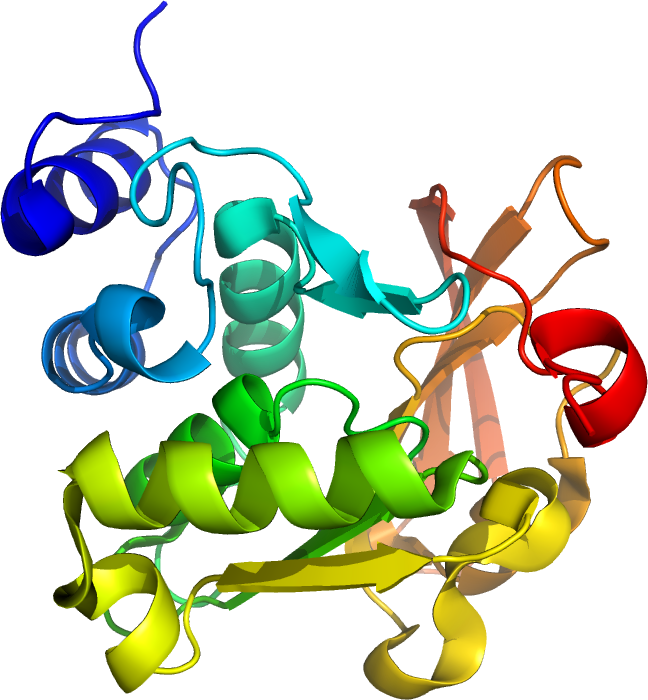
\includegraphics[height=0.25\textheight]{figures/protein.png}%
    \end{tcolorbox}
  \end{tcbraster}
\end{frame}

\begin{frame}{Problems}
  \begin{uugreenbox}[halign=flush center]
    Conditional distribution $\mathbb{P}(Y \,|\, P_X)$ can be \hl{arbitrarily complex}
  \end{uugreenbox}
  \begin{tcolorbox}[blankest, halign=flush center]
    No design choice: e.g., generally not Gaussian even if predictions $P_X$ are Gaussian
  \end{tcolorbox}

  \pause

  \vspace*{1.5\baselineskip}
  \begin{uugreenbox}[halign=flush center]
    \hl{Estimation} of $\mathbb{P}(Y \,|\, P_X)$ is \hl{challenging} (even for classification problems)
  \end{uugreenbox}
  \begin{tcolorbox}[blankest, halign=flush center]
    Usually for each prediction only a single target is observed
  \end{tcolorbox}
\end{frame}

\begin{frame}{Our contributions: Alternative formulation}
  \begin{uubluebox}[halign=flush center]
    A model $P$ is calibrated if $(P_X, Y) \stackrel{d}{=} (P_X, Z_X)$ where $Z_X \,|\, P_X \sim P_X$.
  \end{uubluebox}

  \pause

  Advantages:
  \begin{center}
    \vspace{-\topsep}
    \begin{itemize}
    \item No explicit conditional distributions $\mathbb{P}(Y \,|\, P_X)$
    \item Suggests discrepancy of $\mathbb{P}(P_X, Y)$ and $\mathbb{P}(P_X, Z_X)$
      as calibration measure
    \item Hypothesis testing of calibration is a special two-sample problem
    \end{itemize}
  \end{center}

  \pause
  \begin{center}
    \hl{Applies to any probabilistic predictive model}
  \end{center}
\end{frame}

\begin{frame}{Our contributions: Calibration analysis}
  \begin{center}
    \hl{Estimators and tests of calibration for any probabilistic predictive model}
  \end{center}

  \pause

  \begin{uubluebox}[title={Example: Kernel calibration error (KCE)}]
    \begin{equation*}
      \text{KCE}_k = \text{MMD}_k\big(\mathbb{P}(P_X, Y), \mathbb{P}(P_X, Z_X)\big)
    \end{equation*}
  \end{uubluebox}

  \pause

  \begin{itemize}
  \item No challenging estimation of $\mathbb{P}(Y \,|\, P_X)$
  \item \hl{Marginalization} improves existing (un)biased consistent estimators of the MMD
  \item Generalization of the KCE for classification with more intuitive \hl{real-valued kernels}
  \item Analogous derivation of \hl{calibration tests}
  \end{itemize}
\end{frame}

\begin{frame}{Example: Friedman 1 regression problem}
  \begin{figure}
    \tikzsetnextfilename{experiment}
    \begin{tikzpicture}
      \begin{groupplot}[
        range frame,
        group style={
          group size={2 by 1},
          xticklabels at={edge bottom},
          ylabels at={edge left},
          horizontal sep=0.15\textwidth,
        },
        xlabel=iteration,
        ylabel=estimate,
        height=0.5\textheight,
        width=0.4\textwidth,
        no markers,
      ]
        \nextgroupplot[
          title={NLL},
          y coord trafo/.code={\pgfmathparse{arcsinh(####1)}},
          yticklabel={{$\sinh(\pgfmathprintnumber{\tick})$}},
          legend to name={expleg},
          legend columns={3},
        ]
        \plotstats{NLL}
        \legend{range (train),mean (train),ensemble (train),range (test),mean (test),ensemble (test)}

        \nextgroupplot[
          title={SKCE},
          ymode=log,
        ]
        \plotstats[SKCE (biased)]{SKCE}
      \end{groupplot}
      \node [anchor=north] at ($(group c1r1.west |- group c1r1.outer south)!0.5!(group c2r1.east |- group c2r1.outer south)$){\pgfplotslegendfromname{expleg}};
    \end{tikzpicture}
  \end{figure}

  \begin{uubluebox}[halign=flush center]
    NLL measures both calibration and resolution
  \end{uubluebox}
\end{frame}

\begin{frame}[fragile]{CalibrationErrors.jl and related packages}
  \begin{onlyenv}<1>
    \begin{figure}
      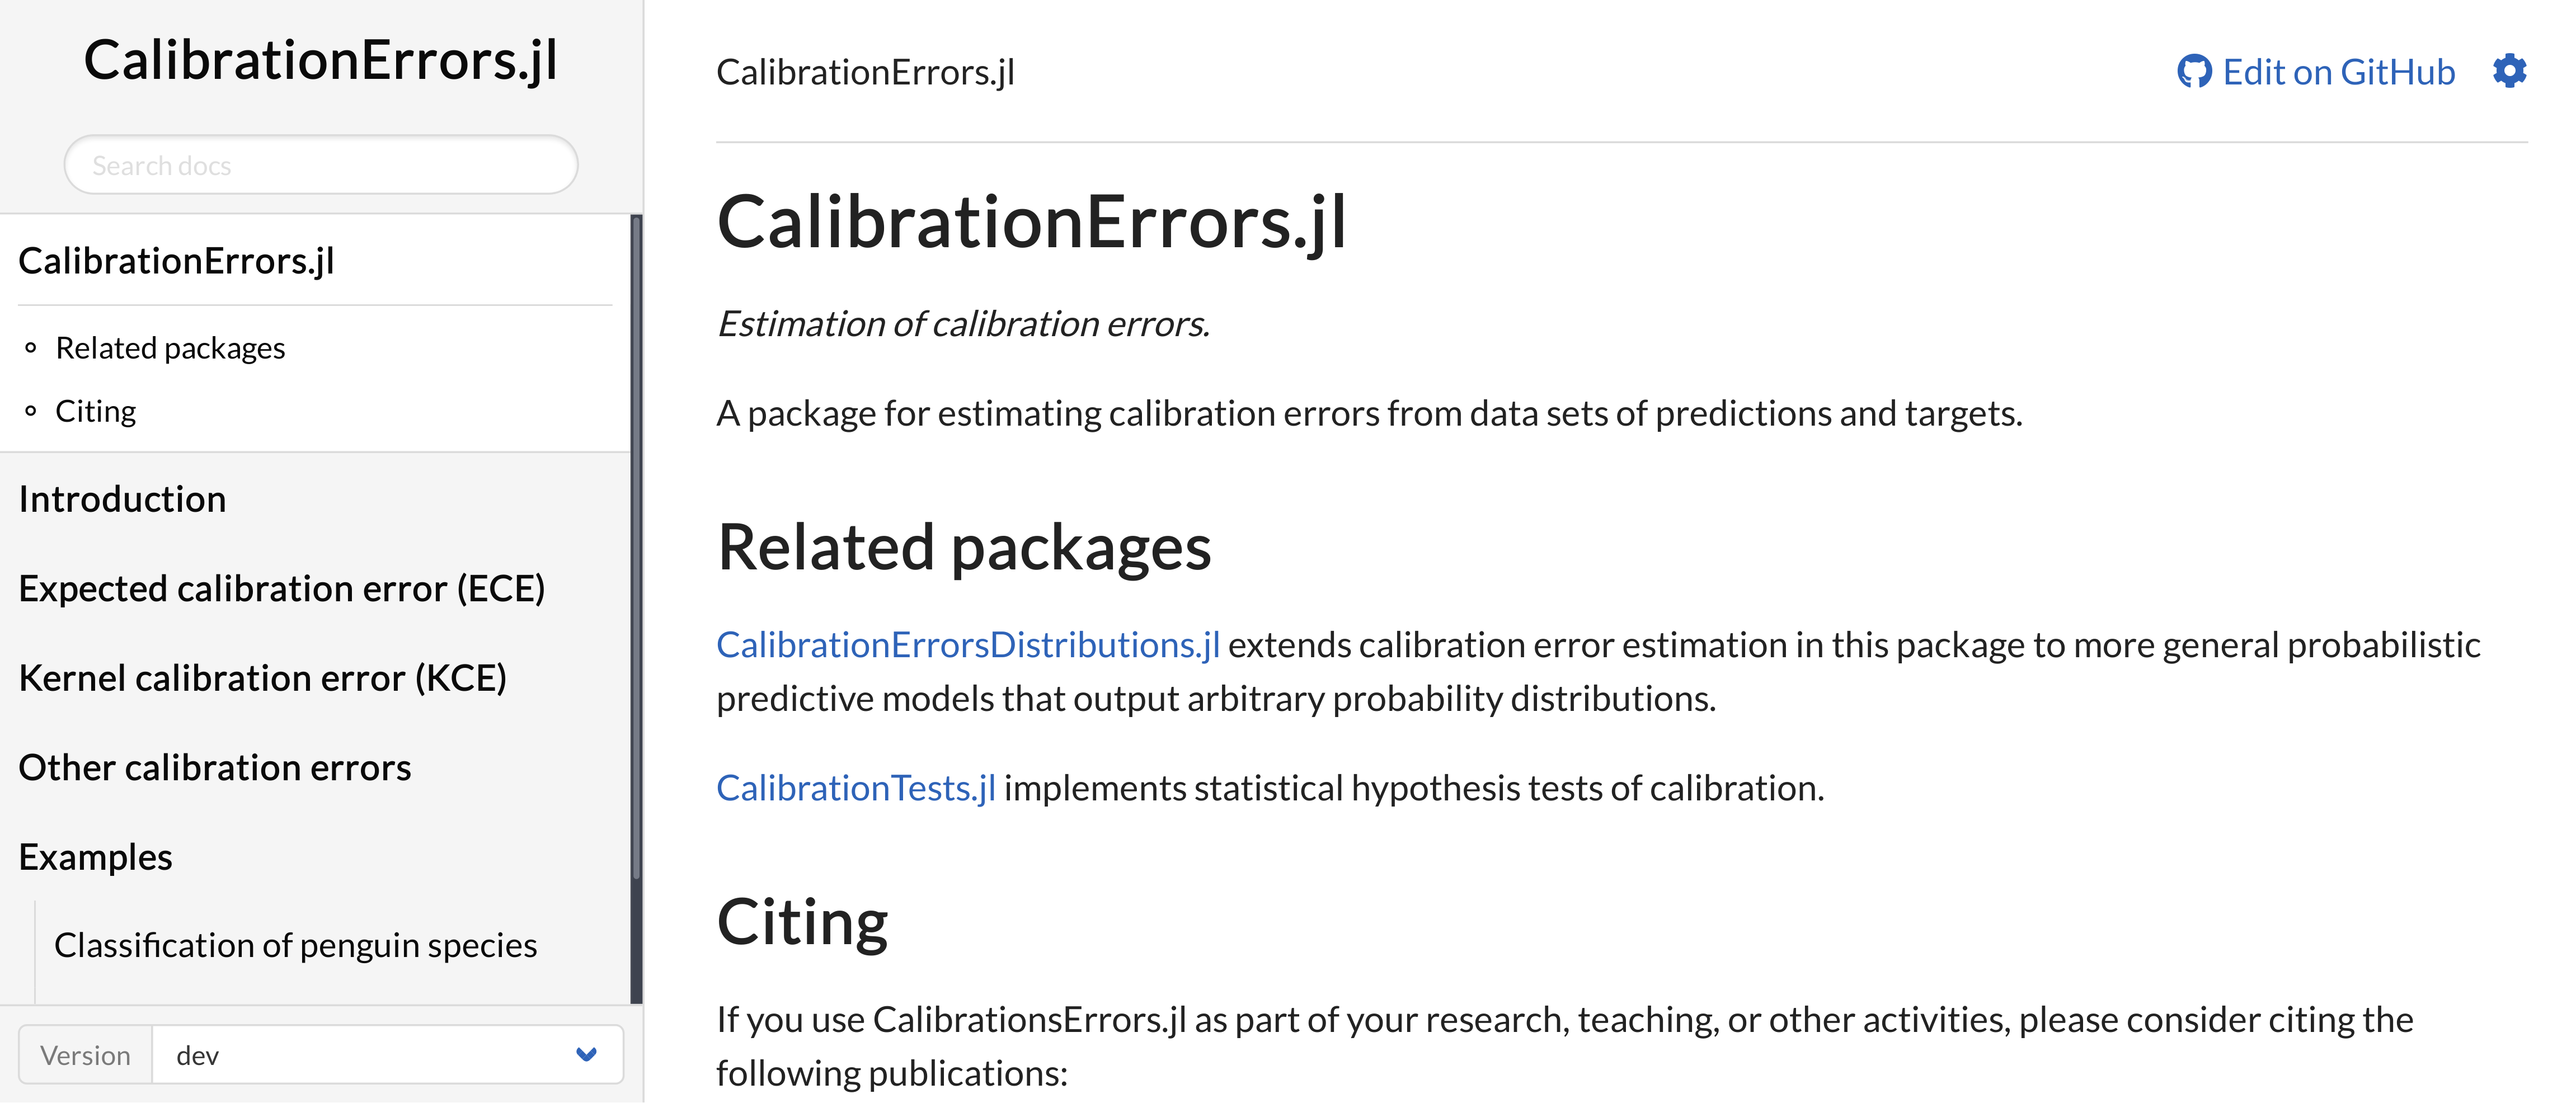
\includegraphics[width=0.9\textwidth]{figures/calibrationerror.png}
    \end{figure}
  \end{onlyenv}
  \begin{onlyenv}<2>
    \begin{juliaconsnippet}
julia> AsymptoticSKCETest(kernel, predictions, targets)
Asymptotic SKCE test
--------------------
Population details:
    parameter of interest:   SKCE
    value under h_0:         0.0
    point estimate:          0.0263758

Test summary:
    outcome with 95% confidence: reject h_0
    one-sided p-value:           <1e-99

Details:
[...]
\end{juliaconsnippet}
\end{onlyenv}
\end{frame}

\begin{frame}[standout]
  \vspace*{2\baselineskip}
	Thank you for listening!\\[2\baselineskip]
  Come see our poster \#2065\\
  May 4th, 8:00am--10:00am UTC
  \vspace*{2\baselineskip}
	\begin{flushleft}
    \normalsize
    Additional material available at:\\
    \url{https://devmotion.github.io/Calibration\_ICLR2021}
	\end{flushleft}
\end{frame}

\end{document}